\chapter{Evaluation Methodology}
\label{chap:evaluation-outline}
\vspace{-0.75cm}
\centerline{\rule{149mm}{.02in}}
\vspace{0.75cm}

The heart of this project is to determine which index structure performs the best for high-dimensional, scientific datasets. Doing this requires an evaluation of the implemented index structures. This section details the measurements and datasets used for evaluation.

\section{Performance Measures}
\label{sec:performance-measures}

The project's core assumptions (see Section \ref{sec:core-assumptions}) state that the target data is dynamic, meaning points may be inserted or deleted at any time. They also state that the project's focus is point query performance. Therefore, index structures are evaluated against the performance of their \textbf{insert}, \textbf{delete} and \textbf{point query} operations. The \textbf{total execution time} of each operation is measured.

The performance of index structures can be affected by their implementations. Therefore, additional measurements will be computed to factor in implementation performance. The first is \textbf{cache miss rate}, which is the rate of cache misses over all CPU reads. A cache miss occurs when the CPU has to fetch data from main memory, which introduces overhead. This overhead can add up and significantly impact the performance of applications.

The second measurement is the \textbf{memory overhead factor}, which measures how much additional memory is needed to store points. An overhead factor of 1 would mean there is no overhead. A factor of 2 would mean \textit{twice} the minimum amount of memory (which is the data required for the actual points) is used. The tools discussed in Section \ref{sec:development-tools} are used to produce some of these measures.

\section{Timing Operations}
\label{sec:timing-operations}

Instead of analysing the performance of a single operation, one can analyse performance of an algorithm over a \textit{sequence} of operations. Amortised analysis, introduced by Tarjan in 1985, is a technique which does this \cite{amortised-analysis}. This type of analysis is typically used for algorithms where some operations take longer than others in order to make future operations quicker. The amortised time complexity of an algorithm describes the \textit{average} runtime of an operation over a sequence of operations. The splay tree, quadtreap and splay quadtree (see Section \ref{sec:history-sensitive-structures}) are examples of index structures that have used amortised analysis to bound the running time of their operations.

This project will use a similar concept for measuring the execution time of the structures. Instead of measuring the time of a single operation, the times of many thousands of operations will be measured. This is to get an idea on what the runtime of an operation is on average, over a sequence of operations. This prevents single, slow operations from causing the execution time to appear worse, or short operations making the performance appear better. Each performance test will invoke the \textbf{Insert-Query-Delete} operation list on each structure, which has the following steps:
\begin{enumerate}
	\item \textbf{Initial Build} -- incrementally build structure by adding each point in test dataset one-by-one
	\item \textbf{Query Points} -- query each point in the dataset
	\item \textbf{Delete Points} -- delete each point in the dataset from the structure until it is empty
\end{enumerate}
Using this process allows the runtime of large numbers of \texttt{insert}, \texttt{delete} and point query operations to be measured. Any performance tests of sequences of operations will be performed five times, and the recorded time will be the \textit{average} of those five times.

\section{Datasets}
\label{sec:datasets}

This section defines the datasets that will be used for the evaluation, which includes both synthetic, artificially generated data and real datasets.

\subsection{Synthetic Datasets}

A variety of point distributions and number of dimensions may tease out the types of data the structures are suited to and which they struggle with. This project uses three kinds of synthetic data, which have uniform, skewed and clustered distributions respectively. Figure \ref{fig:synthetic-data} shows 2D randomly generated points using uniform, skewed and clustered distributions. All generated points are in $[0,1]^d$.

Multiple instances of these datasets will be used, with varying numbers of dimensions. Using such datasets was inspired by Wang et al. and Berchtold et al., who used similar datasets to evaluate the performance of the PK-tree and pyramid tree respectively \cite{pk-tree, pyramid-tree}.

Tu ensure the synthetic data is stastically fair, the Mersenne twister pseudorandom number generator (PRNG) \cite{mersenne-twister} was used to generate the points.  The Mersenne twister passes ``stringent statistical tests" of randomness \cite{mersenne-twister}. The Boost.Random\footnote{\url{http://www.boost.org/doc/libs/1_48_0/doc/html/boost_random.html}} library implements this PRNG. C/C++ have a built-in random number generator, used by invoking the \texttt{rand()} function. Boost.Random was chosen over \texttt{rand()} because the underlying PRNG used by the function is platform-dependent, giving no guarantees it is statistically fair.

Skewed data was generated by applying a power to the number. Let $p$ be a generated point. Since $0 \leq p_i \leq 1$ for all $i \in \lbrace 1, ..., d \rbrace$, this means $p_i^e \leq p_i$ for all $e \geq 1$. This makes smaller values more likely, generating a skewed distribution of points. Increasing $e$ increases the skew. $e = 1.5$ is used to the generate skewed datasets so there are still some points in the upper regions of the data space.

The clustered datasets contain two clusters of points, each contained within the hypercubes $[0,0.5]^d$ and $[0.7,0.8]^d$. There is zero probability that points will appear outside of those cubes.

\begin{figure}
	\begin{center}
		\begin{subfloat}[Uniform Distribution\label{fig:uniform-distribution}]{%
			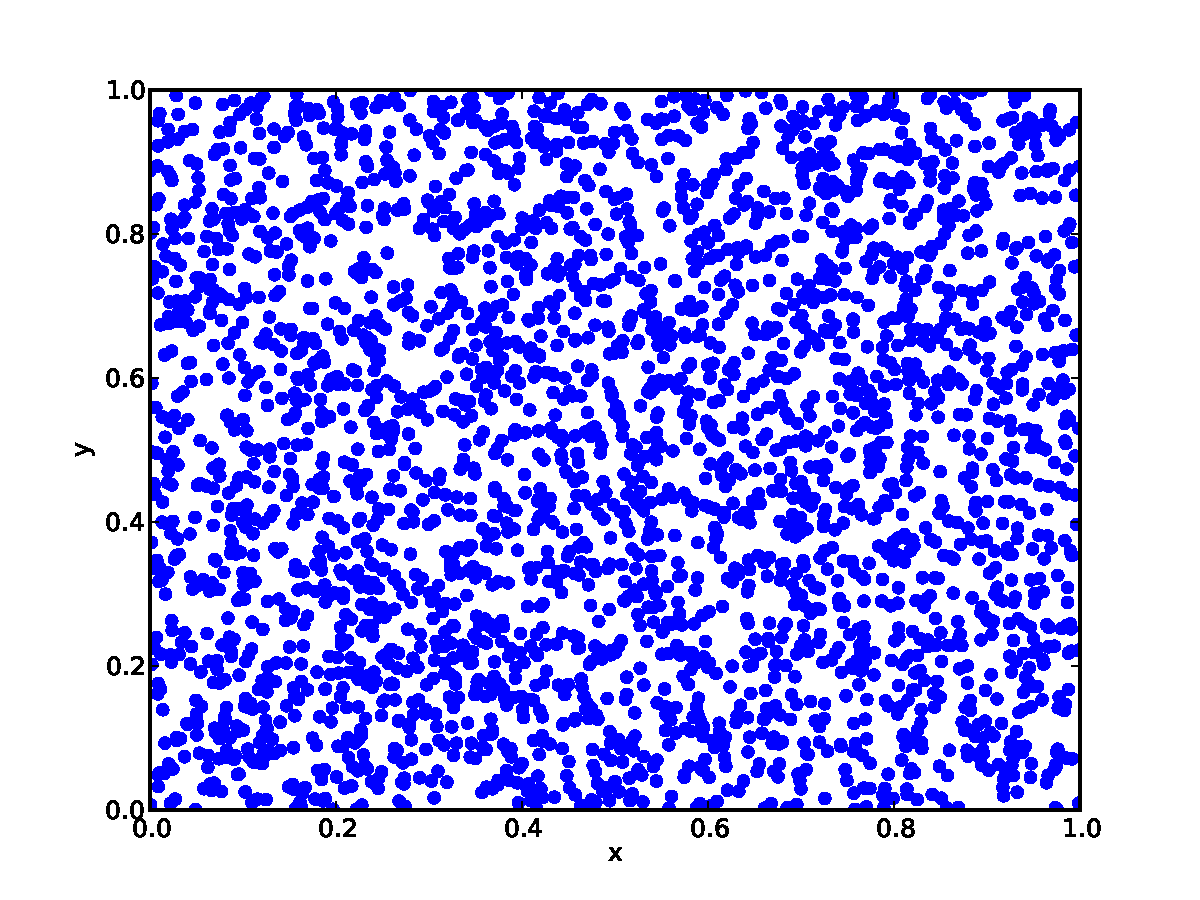
\includegraphics[scale=0.25]{figures/uniform_distribution.pdf}
		}
		\end{subfloat}~
		\begin{subfloat}[Skewed Distribution\label{fig:skewed-distribution}]{%
			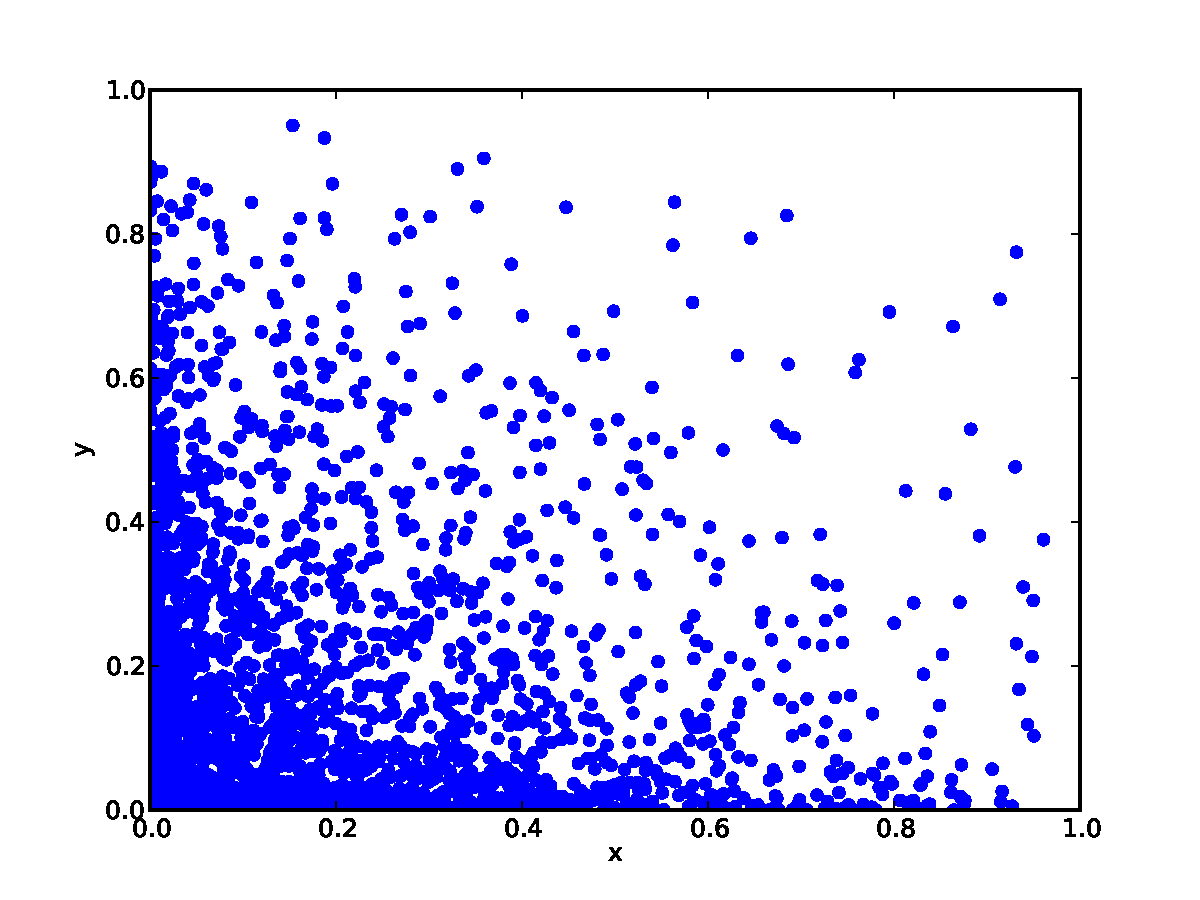
\includegraphics[scale=0.25]{figures/skewed_distribution.pdf}
		}
		\end{subfloat}~
		\begin{subfloat}[Clustered Distribution\label{fig:clustered-distribution}] {%
			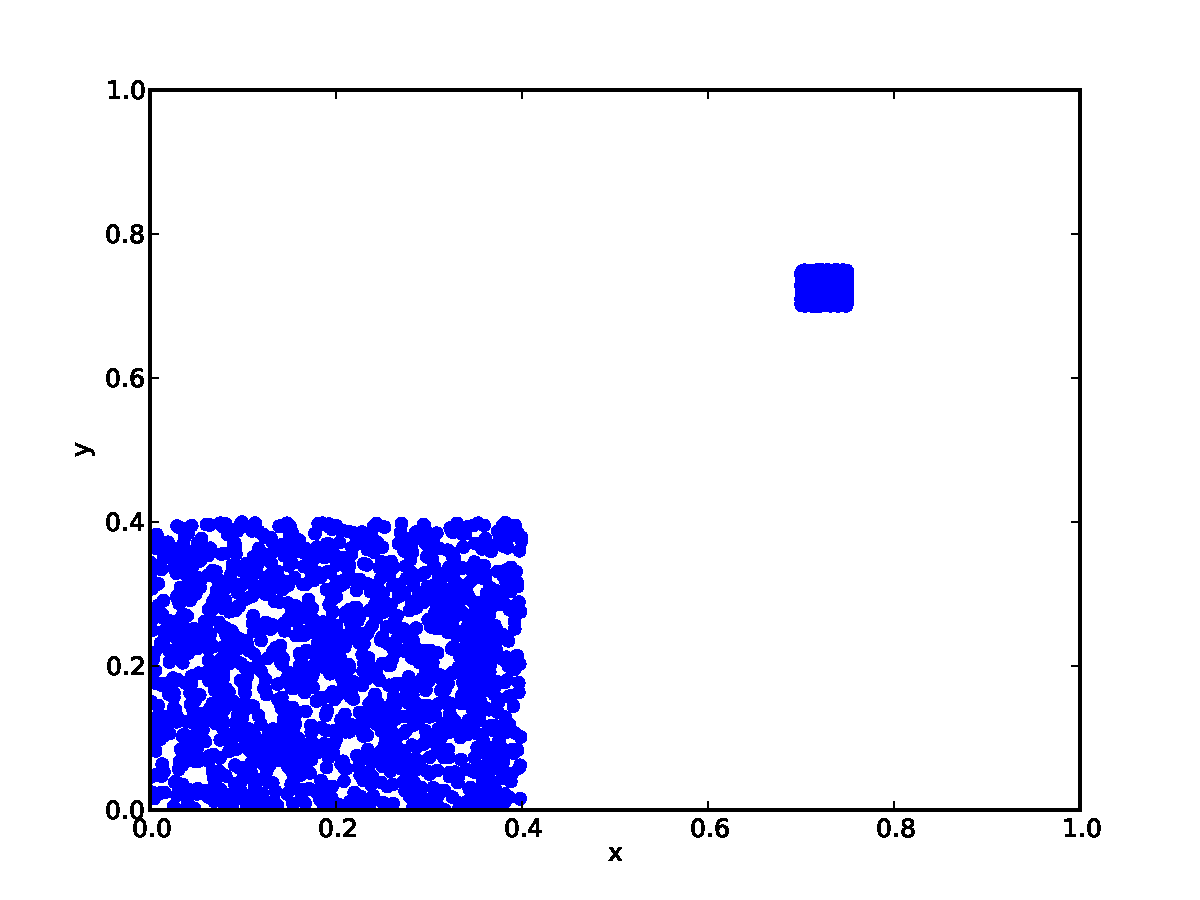
\includegraphics[scale=0.25]{figures/clustered_distribution.pdf}
		}
		\end{subfloat}
	\end{center}

	\caption{Three Types of Synthetic Dataset Used For Evaluation}
	\label{fig:synthetic-data}
\end{figure}

Several synthetic datasets with 10,000 points have been generated for each distribution, varying in dimensionality. The structures will also be evaluated against datasets of varying size. Datasets with different sizes have been generated by sampling from a uniform distribution. These datasets have 16 dimensions to match the Pyramid Tree tests performed by Berchtold et al. in \cite{pyramid-tree}.

\subsection{Real Datasets}

Three real datasets will also be used for the evaluation. The first is the result of an \textbf{astrophysics turbulence simulation}, where a $600 \times 248 \times 248$ regular mesh was used to simulate ``three-dimensional radiation hydrodynamical calculations of ionization front instabilities" \cite{astrophysics-dataset}.  Each point of the mesh has ten scalar fields, which include particle density, temperature and eight chemical species. 200 timesteps were recorded, each being approximately 126 to 128 years apart \cite{astrophysics-dataset}.

A single timestep is used for evaluation, which is timestep 100. This timestep was chosen because there is a greater amount of \textit{``activity"} in the data. The phenomena being modelled starts develop as more time passes, meaning there is greater variance in points. The timesteps near the beginning of simulation are sparse and uniform. Timestep 100 will still contain some amount of sparsity, resulting in dense regions of activity surrounded by relatively sparse, uniform regions. Distributions like this are common in scientific computation, so this timestep should act as a good test on how well the index structures can handle scientific datasets.

The second real dataset contains 13 scalar fields for every point on a $500 \times 100 \times 100$ mesh, over 48 timesteps. It is the result of a simulation of hurricane Isabel from 2003 \cite{hurricane-isabel-dataset}. Timestep 24 of this simulation will be used because, again, the data is highly sparse with dense regions of activity. In the original simulation, nothing was recorded in regions of space that contained ground. The points inside those regions have values of 1.0e+35 to mark they have not been recorded. Since these points given no useful information about the simulation, they have been removed from the dataset.

The astrophysics and hurricane datasets were chosen because they are large and have a high number of dimensions (10 and 13 respectively). The core focus of the project is high-dimensional scientific data, so this data will provide a true test of how well the implementations perform with real instances of such data. Additionally, both datasets are used for scientific visualisation and contain continuous values. As discussed in Section \ref{sec:core-assumptions}, this type of data is what the project is targeting.

Each of these datasets contains millions of points. It was decided that a smaller instance of these datasets would be used, sampling 500,000 points from both datasets. Sampling a sub-region of the grid or uniformly sampling can introduce \textit{bias} in the data, which affects the evaluation. Therefore, smaller instances of the dataset are generated by randomly sampling $n$ points from the original dataset, discarding and picking other points whenever a point that has already been sampled was chosen. The law of large numbers \cite{large-sample-theory} shows that, as the number of samples increase, the sampled dataset starts to become more representative of whole dataset, making this method statistically fairer.

The final real dataset is a point cloud of a 3D armadillo from The Stanford 3D Scanning Repository \cite{armadillo-mesh}, which contains 435,544 points that represent a geometric mesh. This mesh has been used by other researchers to evaluate index structure performance applied to 3D graphics \cite{kd-tree-gpu, accelerating-kdtree-nn}. Appendix \ref{sec:app-real-datasets} shows visualisations of the three real datasets.

Table \ref{tab:operation-lists} lists the evaluation datasets, their size and
dimensionality and lists parameters that will be varied.

\begin{table}
	\centering
	\makebox[\textwidth][c]{%
	\begin{tabular}{|p{4.5cm}|p{3.5cm}|p{2cm}|p{3cm}|}
		\hline
		\textbf{Dataset(s)}
			& \leftspecialcell{\textbf{Fixed} \\ \textbf{Parameter(s)}}
			& \leftspecialcell{\textbf{Varying} \\ \textbf{Parameter}}
			& \textbf{Parameter Values}  \\
		\hline
		Uniform, Skewed, Clustered & 10,000 Points & Dimension & \leftspecialcell{1, 2, 3, 5, 10, \\ 50, 100, 200} \\
		\hline
		16D Uniform & 16 dimensions & Input Size & \leftspecialcell{10,000, 100,000, \\ 500,000} \\
		\hline
		Astrophysics ($t = 100$) & \leftspecialcell{10 dimensions, \\500,000 points} & - & - \\
		\hline
		Hurricane Isabel ($t = 24$)& \leftspecialcell{13 dimensions, \\500,000 points} & - & - \\
		\hline
		Armadillo Mesh & \leftspecialcell{3 dimensions, \\435,544 points} & - & -\\
		\hline
	\end{tabular}}%
	\caption{Evaluation Datasets}
	\label{tab:operation-lists}
\end{table}

\section{Environment}

Table \ref{tab:system-specifications} lists the hardware, operating system and tool versions used to implement the index structures and measure their performance. 

\begin{table}
	\centering
	\begin{tabular}{|r|l|}
		\hline
		\textbf{CPU} & Intel(R) Xeon(R) CPU E3-1225 V2 @ 3.20 GHz (four cores) \\
		\hline
		\textbf{Main Memory (RAM)} & 15.5 GB \\
		\hline
		\textbf{Operating System} & Linux CentOS 6.5 (Final) \\
		\hline
		\textbf{Linux Kernel Version} & 2.6.32-431.3.1.el6.x86\_64 \\
		\hline
		\textbf{C++ Compiler} & GCC 4.4.7 (Released 13/03/2013) \\
		\hline
		\textbf{Boost Library Version} & 1.41.0 \\
		\hline
	\end{tabular}
	\caption{Hardware, OS and Tool Versions Used for Development and Performance Testing}
	\label{tab:system-specifications}
\end{table}

\subsection{Measuring Execution Time}

Individual index structure operations are typically much lower than a second, sometimes even less than a millisecond. A high level of precision and accuracy is required because even millisecond savings are important when optimising index structures.

C/C++ comes with two standard timing mechanisms. \texttt{time()}\footnote{Online documentation for discussed functions at: \url{http://www.cplusplus.com/reference/}} returns the number of seconds since the Unix epoch (00:00, 01/01/1970 UTC). \texttt{clock()} measures the number of CPU ticks since some epoch (typically the launch of the application). The amount of real time (i.e. milliseconds, seconds, etc.) a CPU tick takes is constant, but depends on the hardware. \texttt{clock\_gettime()} returns a time with nanosecond precision, but is only available on specific systems (e.g. Linux). Since the operating system used for the evaluation framework is a Linux distribution and nanosecond precision is desired, \texttt{clock\_gettime()} has been used for timing all operations.

\section{Initial Hypothesis}
\label{sec:initial-hypothesis}

Since there has been no published evaluations of the Pseudo-Pyramid Tree or Bit Hash, no hypotheses will be made regarding the performance of these structures. It is suspected that the Pseudo-Pyramid Tree will perform well on high-dimensional data, because it is a hash-based method, but little is currently known about how well the structure's hashing function performs, so there is a little basis for such suspicion. Based on the reported performance of the Pyramid Tree and $kd$-tree in a high-dimensional setting in the literature (discussed in Chapters \ref{chap:background_research} and \ref{chap:chosen-structures}), the following hypothesis was devised:

\paragraph{\textbf{HYPOTHESIS:}} Pyramid Tree will be faster than the baselines and $kd$-trees on scientific datasets containing high-dimensional data ($\geq 10$ dimensions).

\paragraph{}

After the performance evaluation, the hypothesis will be revisited to determine if it still holds, and \textit{why} it does or does not hold will be explored.

\section{Conclusion}

TODO